\section{Models and Methods}

\subsection{Data acquisition model}

Assume we have linked-reads composed of $m$ barcodes, coming from $n$ molecules, obtained from a larger molecule $M$ (say a chromosome) of length $L$. We denote by $\Balph{}$ the barcode alphabet, $|\Balph|=m$ and by $B$ the mapping associating to a molecule its barcode.
We introduce some simplifying assumptions: no molecule is fully included into another one, no two molecules have the same starting coordinate, consecutive molecules along $M$ do overlap. 
This allows us to see the sequenced molecules as discrete intervals over $[1,2n]$ and implies that there is a total order $\MolOrd{}$ of these molecules (ordered by increasing starting coordinate); we denote by $M_1,\dots,M_n$ these molecules, with $M_i$ being the $i^{th}$ molecule in the order $\MolOrd$.
In this setting, we do not consider as intersecting a molecule whose endpoint is in discrete coordinate $i$ and a molecule whose start is in coordinate $i$.
Finally we assume through these notes that every molecule, but the last and first ones along $M$, does intersect at least two other molecules, a realistic assumption of coverage of the sequencing experiment.

\subsection{Graph-theoretic formulation}

\textbf{Intersection graphs.} An undirected graph $G=(\{v_1,\ldots,v_n\},E)$ is an \emph{intersection graph} if a set $S_i$ can be assigned to each node $v_i$, such that an arc $(v_i,v_j)$ exists if and only if $S_i \cap S_j \neq \emptyset$. All undirected graphs are intersection graphs.

\noindent \textbf{Interval graphs.} An \emph{interval graph} is an intersection graph where all the $S_i$'s are single continuous intervals.

\noindent \textbf{Barcode sequence.}
In reference to the data acquisition model, we denote by $B(\MolOrd)$ the projection of $\MolOrd{}$ over $\Balph{}$ obtained by replacing each $M_i$ in $\MolOrd{}$ by its barcode; we call this sequence the \textit{true barcode sequence}.


\begin{problem}[Molecule counting]
    \label{def:problem1}
    Let  $B(\MolOrd)$ be a true barcode sequence. For each molecule $M_i$, determine the number of occurrences of $M_i$ in  $B(\MolOrd)$.
\end{problem}

\noindent \textbf{Barcode intersection graph} The graph $G_b=(V,E)$ where $V=\Balph{}$ (so $|V|=m$) and ${x,y}\in E$ iff barcodes $x$ and $y$ contain intersecting molecules $M_i \in x$ and $M_j\in y$ where intersection is defined in terms of genomic coordinates. 
Note that this graph can have multiple edges (multi-edges) and loops and is connected (by our assumption of consecutive molecules overlapping). 

\begin{property}
    \label{prop:simple} The true barcode intersection graph is a simple graph if and only if there does not exist (1) intersecting molecules $M_i$ and $M_j$ such that $B(M_i)=B(M_j)$ and (2) intersecting molecules $M_i, M_j$ and intersecting molecules $M_k,M_\ell$ such that $B(M_i)=B(M_k)$ and $B(M_j)=B(M_\ell)$. 
\end{property}

The property above is immediate, but it implies that if $n$ is large enough, that (1) the length of the molecules and (2) the number of molecules per barcode can be considered as constant, then we can expect, with high probability, that the true barcode intersection graph is simple, and the edge set of $G_b$ is in bijection with the edges set of the molecules intersection graph (in other words, collapsing molecules into barcodes did not create multi-edges or loops). In the following, we will seek to study whether this property is satisfied in real-life instances.



\begin{problem}[Molecule order recovery from a true barcode intersection graph]
    \label{def:problem2}
    Let $G_b$ be a true barcode intersection graph. Compute a walk $W$ in $G$ such that the sequence of visited vertices $V(W)$ is equal to the true barcode sequence $B(\MolOrd)$.
\end{problem}

\subsection{Barcode graph structure}

Here we can focus on Cedric Analysis (O2, O3 and On ?).

\subsection{$d$-graphs: underlying local graph structure}
prerequisite to this section: Description of the merging process (DONE), underlying intersection graph (DONE), long molecule overlap efficiency. 


% another definition of d-graph
%\noindent \textbf{$d$-graph.} We introduce the notion of a \emph{$d$-graph}, for even values $d\geq 2$, which is an interval graph such that: i) no interval is strictly included in another, and ii) every interval intersects with exactly $d/2$ intervals to the left and $d/2$ intervals to the right. 
%Immediate properties of a $d$-graph are: 1) each vertex has exactly $d/2$ in-neighbors and $d/2$ out-neighbors, 2) a transitively reduced $d$-graph is a path.
%%%If we ignore that intervals assigned to nodes, a $d$-graph is just a path graph, where $d-2$ transitive edges are added to the extended neighborhood of each node. %A $d$-graph can also be seen as an unlabeled graph, independently of the underlying intervals. %But it will help to remind oneself that $d$-graphs are interval graphs.

\subsubsection*{$d$-graphs and the effect of barcode collisions}

As a first approximation, consider an interval graph of molecules (termed \emph{molecule graph} and later abbreviated as $MG$) that is \emph{ideal} in the following sense: molecules have identical sizes, are evenly-spaced along the genome, and all the overlaps across their respective genomic intervals (and only those) are detected.
Such interval graph is represented on the Fig-\ref{fig:fusion}(a). 

\textbf{Remark 1}: %If each of the molecules is uniquely aligned on the genome,  %hypothèse ajoutée à 'ideal' au dessus
each node of the MG is strongly connected to local nodes\footnote{ 'local nodes' est ambigu. 'neighbors' plutot?} and disconnected from the rest of the MG. The more molecules are overlapping each other,  the more the "edge thickness" is high\footnote{problematique car 'edge thickness' n'est pas defini}.\\

Given a molecule, we denote by \textit{depth} ($d$) the number of other molecules that the molecule intersects with. To avoid edge effects, we will consider that the genome is circular. For example, if at any a given genome position exactly 4 molecules overlap this position, then all molecules have depth $d=3$.

\noindent \textbf{$d$-graphs.} We call $d$-graph an interval graph where $d$ is constant everywhere except for the $d$ leftmost and rightmost nodes.

During the sequencing process, having a barcode collision between two molecules means merging two nodes from the MG (Fig-\ref{fig:fusion}-b) into one node $c$ in the barcode graph (BG).
Because the MG is thick\footnote{undefined notion}, even if the molecule information itself is lost during the merging process, the edges around $c$ are conserved.
These edges are clues to reconstruct the molecules\footnote{.. order?}.
If there is no other "local"\footnote{need to cleanly define what is a local fusion before this sentence} fusion (ie no two molecules from the direct neighborhood of c are merging together), the molecule provenance information can be reconstructed by studying the edges\footnote{need to reformulate this sentence because it is informal, e.g. 'we will later see that molecule order can be inferred despite this fusion having been made'}.

\begin{figure}[htp]
    \centering
    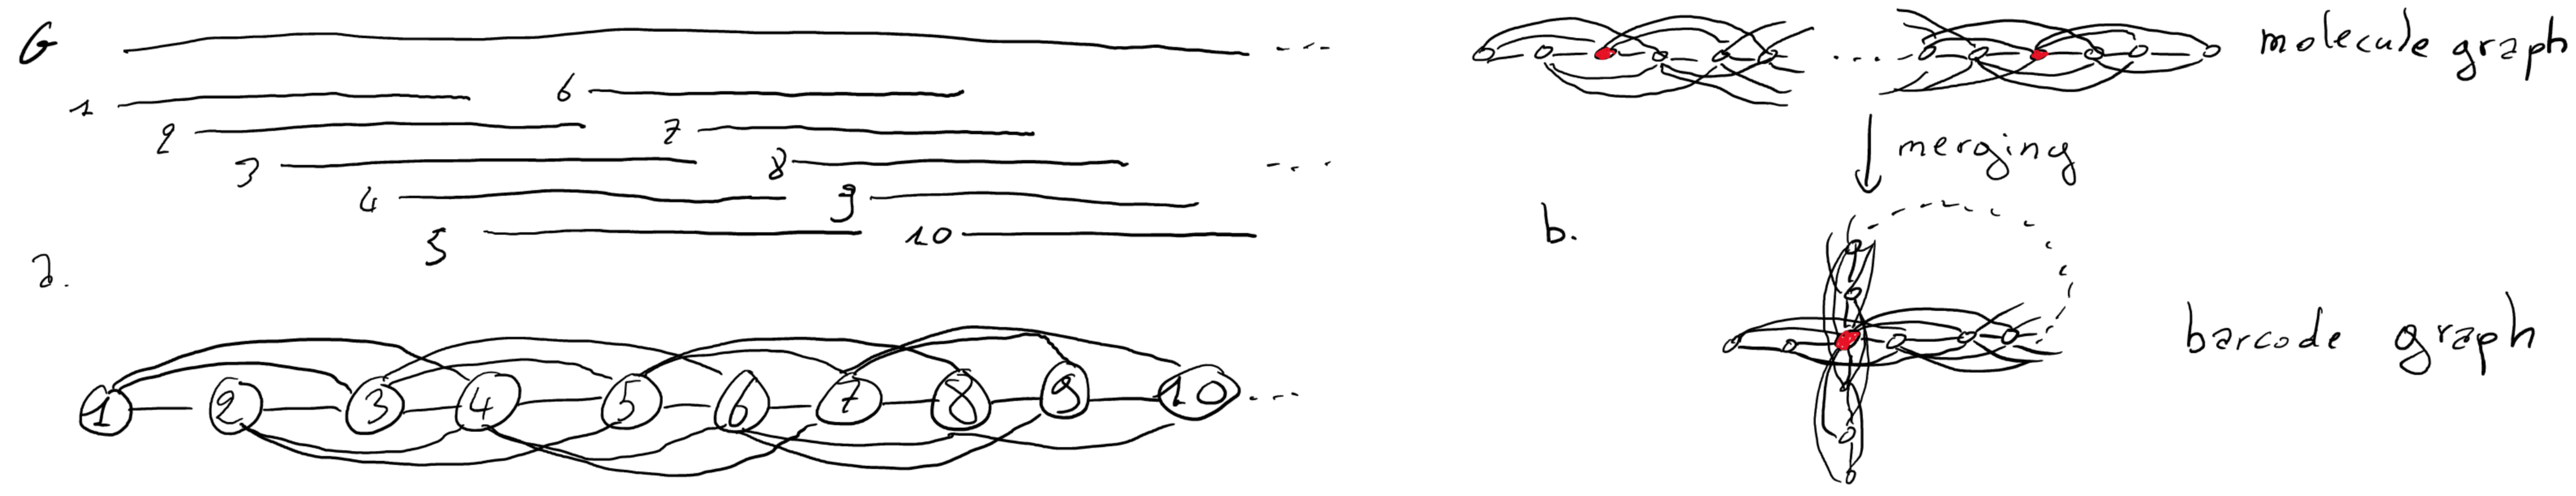
\includegraphics[width=\textwidth]{fusion.pdf}
    \caption{ a. (top) An alignment of long molecules to a genome $G$. (bottom) A representation of the interval graph from aligned molecules to the genome $G$. b. The fusion of two nodes (red barcode) from the molecule graph, preserve edge orientations in the barcode graph. }
    \label{fig:fusion}
\end{figure}

\footnote{Rayan: j'en suis là de ma passe de remarques}

\subsubsection*{The building blocks of the $d$-graphs}

From a $d$-graph, extract a node (not in the $d$ nodes from the extreme positions in the graph), its $2\times d$ neighbors and all the induced edges.
We call this subgraph a \textit{unit $d$-graph} (udg).
Because we are in the perfect conditions, each of the nodes (excluding extreme nodes) induce an udg.
So udgs are the building blocks of a $d$-graph.

In the figure \ref{fig:perfect_udg}, we represented an extracted udg from its context.
From the bottom representation, we can see the different components of an udg.
First, an udg is composed of exactly $2\times d + 1$ nodes and centered on a node $c$.
All the other nodes are in the direct neighborhood of $c$ (the blue edges).
These $2 \times d$ nodes are 2 cliques of size $d$ (black edges).
Finally, the cliques are bounded together by what we call \textit{linking edges} (red edges).\\
\textbf{Remark}: From left to right on the representation, the linking edge number bounded\footnote{bounded=?} to a node increase from 0 to $d-1$ before the central node ; then decrease from $d-1$ for the node just after $c$ to 0 for the rightmost node.
On total, there is exactly $\sum_{i=0}^{d-1}i$ linking edges in a udg.\\

\begin{figure}[htp]
    \centering
    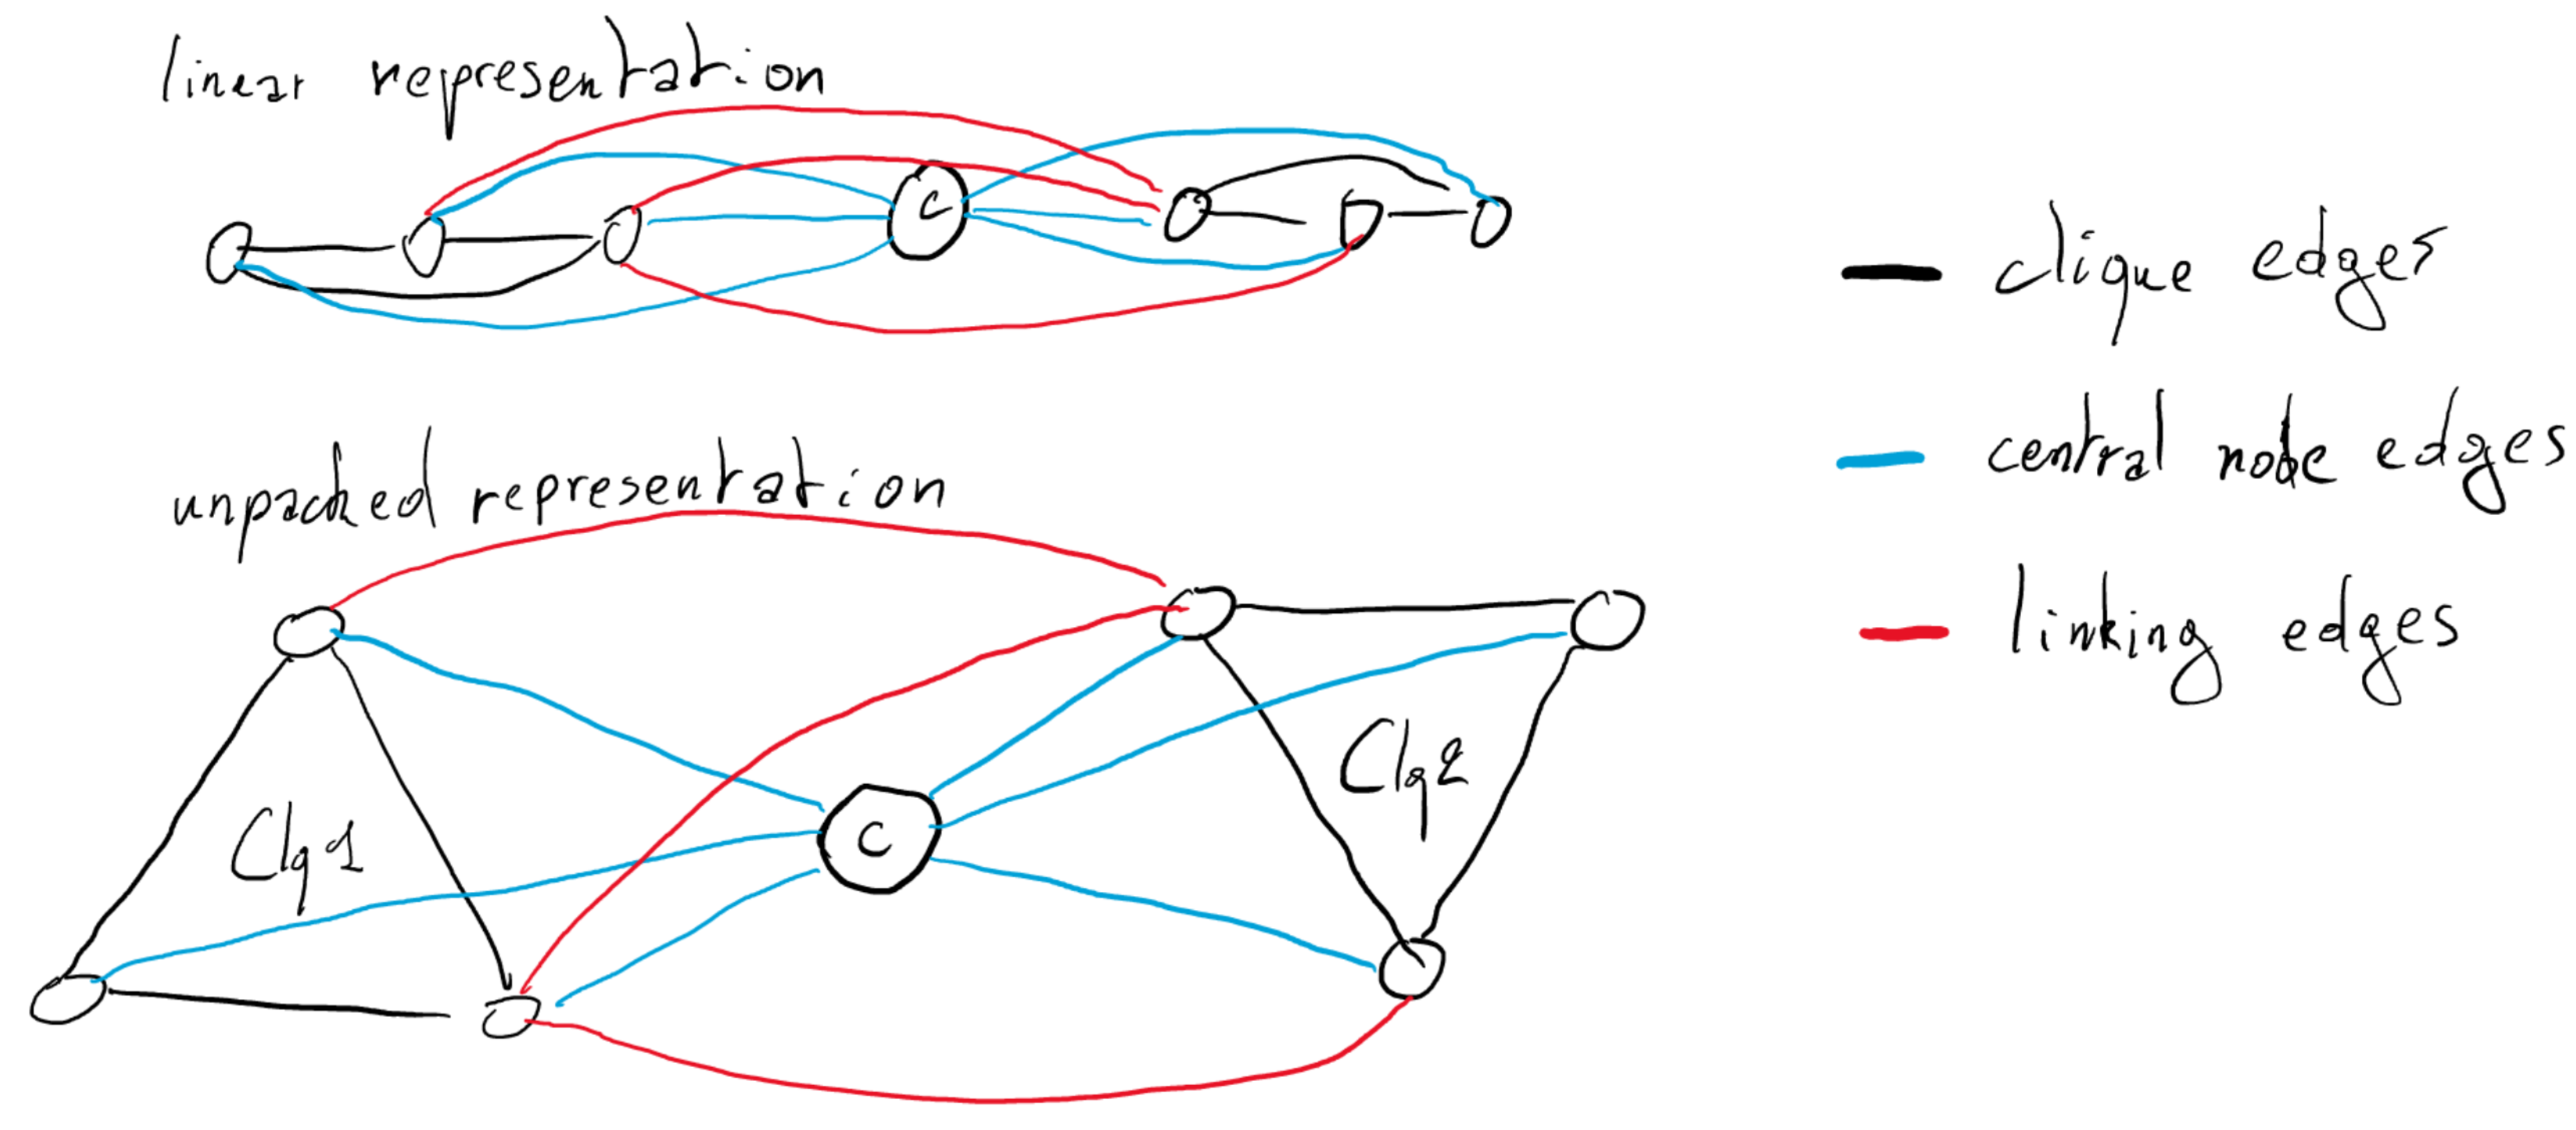
\includegraphics[width=0.7\textwidth]{udg_composition.pdf}
    \caption{A unit 3-graph. Linear representation on top, unpacked representation on bottom. $c$ node is the central node. In black, the edges from the side cliques of the unit 3-graph. In blue, the edges between the central nodes and the other nodes. In red, the edges that bound the side cliques together.}
    \label{fig:perfect_udg}
\end{figure}

The representation of a $d$-graph as a succession of overlapping unit $d$-graphs is very important to transform the problem of "searching a $d$-graph into an intersection graph"\footnote{pas compris ce probleme} to "searching a path into a set of unit $d$-graphs".
So, the first step to our $d$-graph reconstruction is to find a set of udgs inside of the BG.

\subsubsection*{Compute the udgs from a Barcode Graph}

The elements entering in the composition of a udg are used to extract them from their BG context.
For each node of the BG we apply the algorithm \ref{algo:udg}.

\begin{algorithm}
    \caption{Unit $d$-graph computation}
    \label{algo:udg}
    \begin{algorithmic}[1] % The number tells where the line numbering should start
        \Procedure{compute\_udg}{$n, d, BG$} \Comment{n: start node}
            \State $U \gets$ \O
            \State $nbs\gets BG.neighbors(n)$
            \State $subgraph \gets BG.induced\_subgraph(nbs)$
            \State $cliques \gets subgraph.cliques(d)$ \Comment{list cliques of size d}
            \For{$c1 \in cliques$}
                \For{$c2 \in cliques$}
                    \State $c \gets count\_links(c1, c2)$ \Comment{Count edges between the cliques}
                    \If{$c == \sum_{i=0}^{d-1}i$}
                        \State $U \gets U \cup udg(n, c1, c2)$ \Comment{Add the new udg}
                    \EndIf
                \EndFor
            \EndFor
            \State \textbf{return} $U$
        \EndProcedure
    \end{algorithmic}
\end{algorithm}


The central node is used to perform only a local search, the cliques are searched independently and the linking edges are used to confirm the presence of a unit $d$-graph.
If there is no local multiple fusion, this algorithm is sufficient to discover all the unit $d$-graphs (\textbf{Proof ?}).

\subsubsection*{Compute udgs on real Barcode Graphs}

Real barcode graphs are not $d$-graphs. They differ in the following key aspect: molecule depth, and molecule length, vary along the genome. As a result, the depth $d$ is no longer constant unlike in our previous idealized model.

\textbf{Hypothesis 1}: it's more probable that $d$ smoothly vary along thousands of nucleotides rather than quickly drop or jump on a few base pair.\\
To avoid explicit use of the $d$ value in the udg computation process, we adapted algorithm \ref{algo:udg} to compute pseudo-udgs instead of perfect udgs.\\
\textbf{Hypothesis 2}: local max-cliques are a good proxy to $d$-cliques because the random fusion process should not repetitively merge together nodes from 2 (or more) local neighborhoods. Complete destructive fusions are highly improbable.\\
\textbf{Remark:} If the previous hypothesis is not true, there is a local critical merge.
The local information is lost and some udgs can't be computed but the other nodes can still be deconvoluted.

Without the $d$ value, we don't have a precise criteria to say that 2 cliques are the hands of a udg.
Instead, we score the approximated udgs by their linking edge count divergence from the count for an equivalent well balanced udg.
We use the algorithm \ref{algo:score} to score a pair of cliques.

\begin{algorithm}
    \caption{Divergence score between two cliques}
    \label{algo:score}
    \begin{algorithmic}[1] % The number tells where the line numbering should start
        \Procedure{div}{$c1, c2$} \Comment{cliques can be of different size}
            \State $d \gets max(|c1|, |c2|)$ \Comment{d used is the max length of cliques}
            \State $ref \gets \sum_{i=0}^{d-1}i$
            \State $obs \gets count\_links(c1, c2)$
            \State \textbf{return} $\sqrt{(ref - obs)^2}$ \Comment{Absolute difference}
        \EndProcedure
    \end{algorithmic}
\end{algorithm}

From this divergence score, one way to compute udgs is to fix a threshold and only generate a udg if its clique divergence is lower than that threshold.
But this solution is not sufficient to handle all $d$ values and variations.
Using it, results in producing too much or too few udgs regarding the threshold value.

\subsubsection*{Approximating the number of udgs}

To create only good udgs, we want to pair cliques that involve good divergence score.
So, first, from the list of all the max cliques computed on the neighborhood of a central node, we create a complete graph of cliques where the nodes are the cliques and the edges are weighted with the linked cliques divergence score (see figure \ref{fig:mwm}).\\
\textbf{Hypothesis 1}: No max clique is present inside of two different udg.\\
\textbf{Remark}: If the previous hypothesis is wrong for a $k$-clique, that means that in two different place of the genome, $k$ overlapping molecules share the same $k$ barcodes. It's highly improbable for large $k$ values.\\
\textbf{Hypothesis 2}: All the max cliques will be part of an interesting udg. This hypothesis is not totally true but will lead to an almost perfect solution that will be filtered in the following sections.

\begin{figure}[htp]
    \centering
    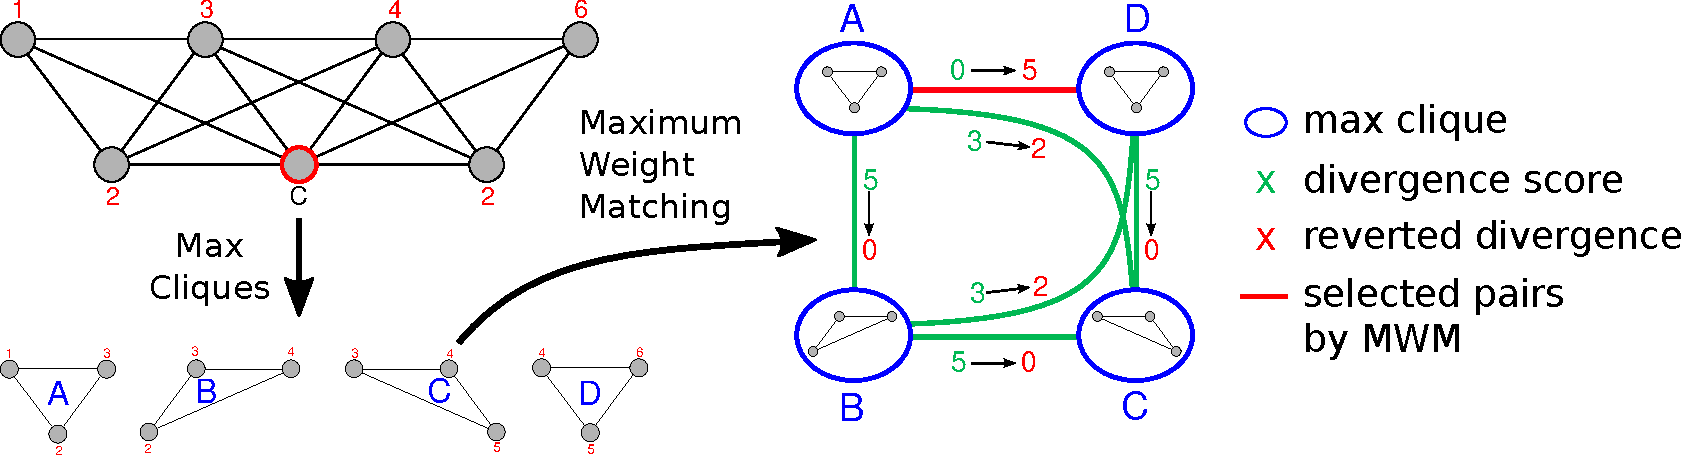
\includegraphics[width=\textwidth]{mwm.pdf}
    \caption{Max clique graph construction and maximum weight matching application}
    \label{fig:mwm}
\end{figure}

Regarding the two hypothesis, we created a udg factory based on the maximum weight matching algorithm.
This algorithm produce a matching in the graph, where the sum of all the selected edges weight is maximal.
In our clique graph we want the edges that are minimum.
So, we revert the maximum divergence order by doing $max\_div - div$ on each node. max\_div is the maximal divergence score on all the local clique pairs (see Fig. \ref{fig:mwm}).

\begin{algorithm}
    \caption{Approximate unit $d$-graph computation}
    \label{algo:audg}
    \begin{algorithmic}[1] % The number tells where the line numbering should start
        \Procedure{compute\_udg}{$n, BG$} \Comment{n: start node}
            \State $U \gets$ \O
            \State $nbs\gets BG.neighbors(n)$
            \State $subgraph \gets BG.induced\_subgraph(nbs)$
            \State $cliques \gets subgraph.max\_cliques()$ \Comment{list cliques of maximum size}
            \State $CG \gets clique\_graph(cliques)$ \Comment{Clique graph from divergences}
            \State $m = CG.maximum\_weight\_matching()$
            \For{$(c1, c2) \in m$}
                \State $U \gets U \cup udg(n, c1, c2)$ \Comment{Add the new udg}
            \EndFor
            \State \textbf{return} $U$
        \EndProcedure
    \end{algorithmic}
\end{algorithm}

The final algorithm to compute the approximate unit $d$-graphs is presented in algorithm \ref{algo:audg}.
It is now totally independent of the $d$ values.
The usage of a maximum weight matching on our clique graph generate high quality udgs but don't have a guaranty on correctness of those udgs.

Local search for linked cliques are a kind of local graph community detection.
More than classical clustering, the max clique detection allow to include some nodes in multiple communities.
This property leads to a udg detection algorithm very resilient to multiple local merges.
But because we use a heuristic to generate udgs some of them are wrong and others are missing.

\subsection{$d^{2}$-graph: Connecting unit $d$-graphs}

In this section, we will use unit $d$-graph or udg as language shortcut for what we called approximate unit $d$-graph in the previous sections.
We will use \textit{perfect udg} for a well balanced and 0 divergence udg.

udgs are local structure defined in a node neighborhood in the barcode graph.
Because we know that the barcode graph is originated from an intersection graph, we should be able to find a succession of udg that cover our genome from the beginning to the end.
In fact, if we are in the perfect case, the genome should be a succession of perfect udgs where two successive udg share exactly $2 \times d$ barcodes.
Each of the two udgs will have one barcode that is not in the other.
We can call these two nodes \textit{extreme nodes}.

\begin{figure}[htp]
    \centering
    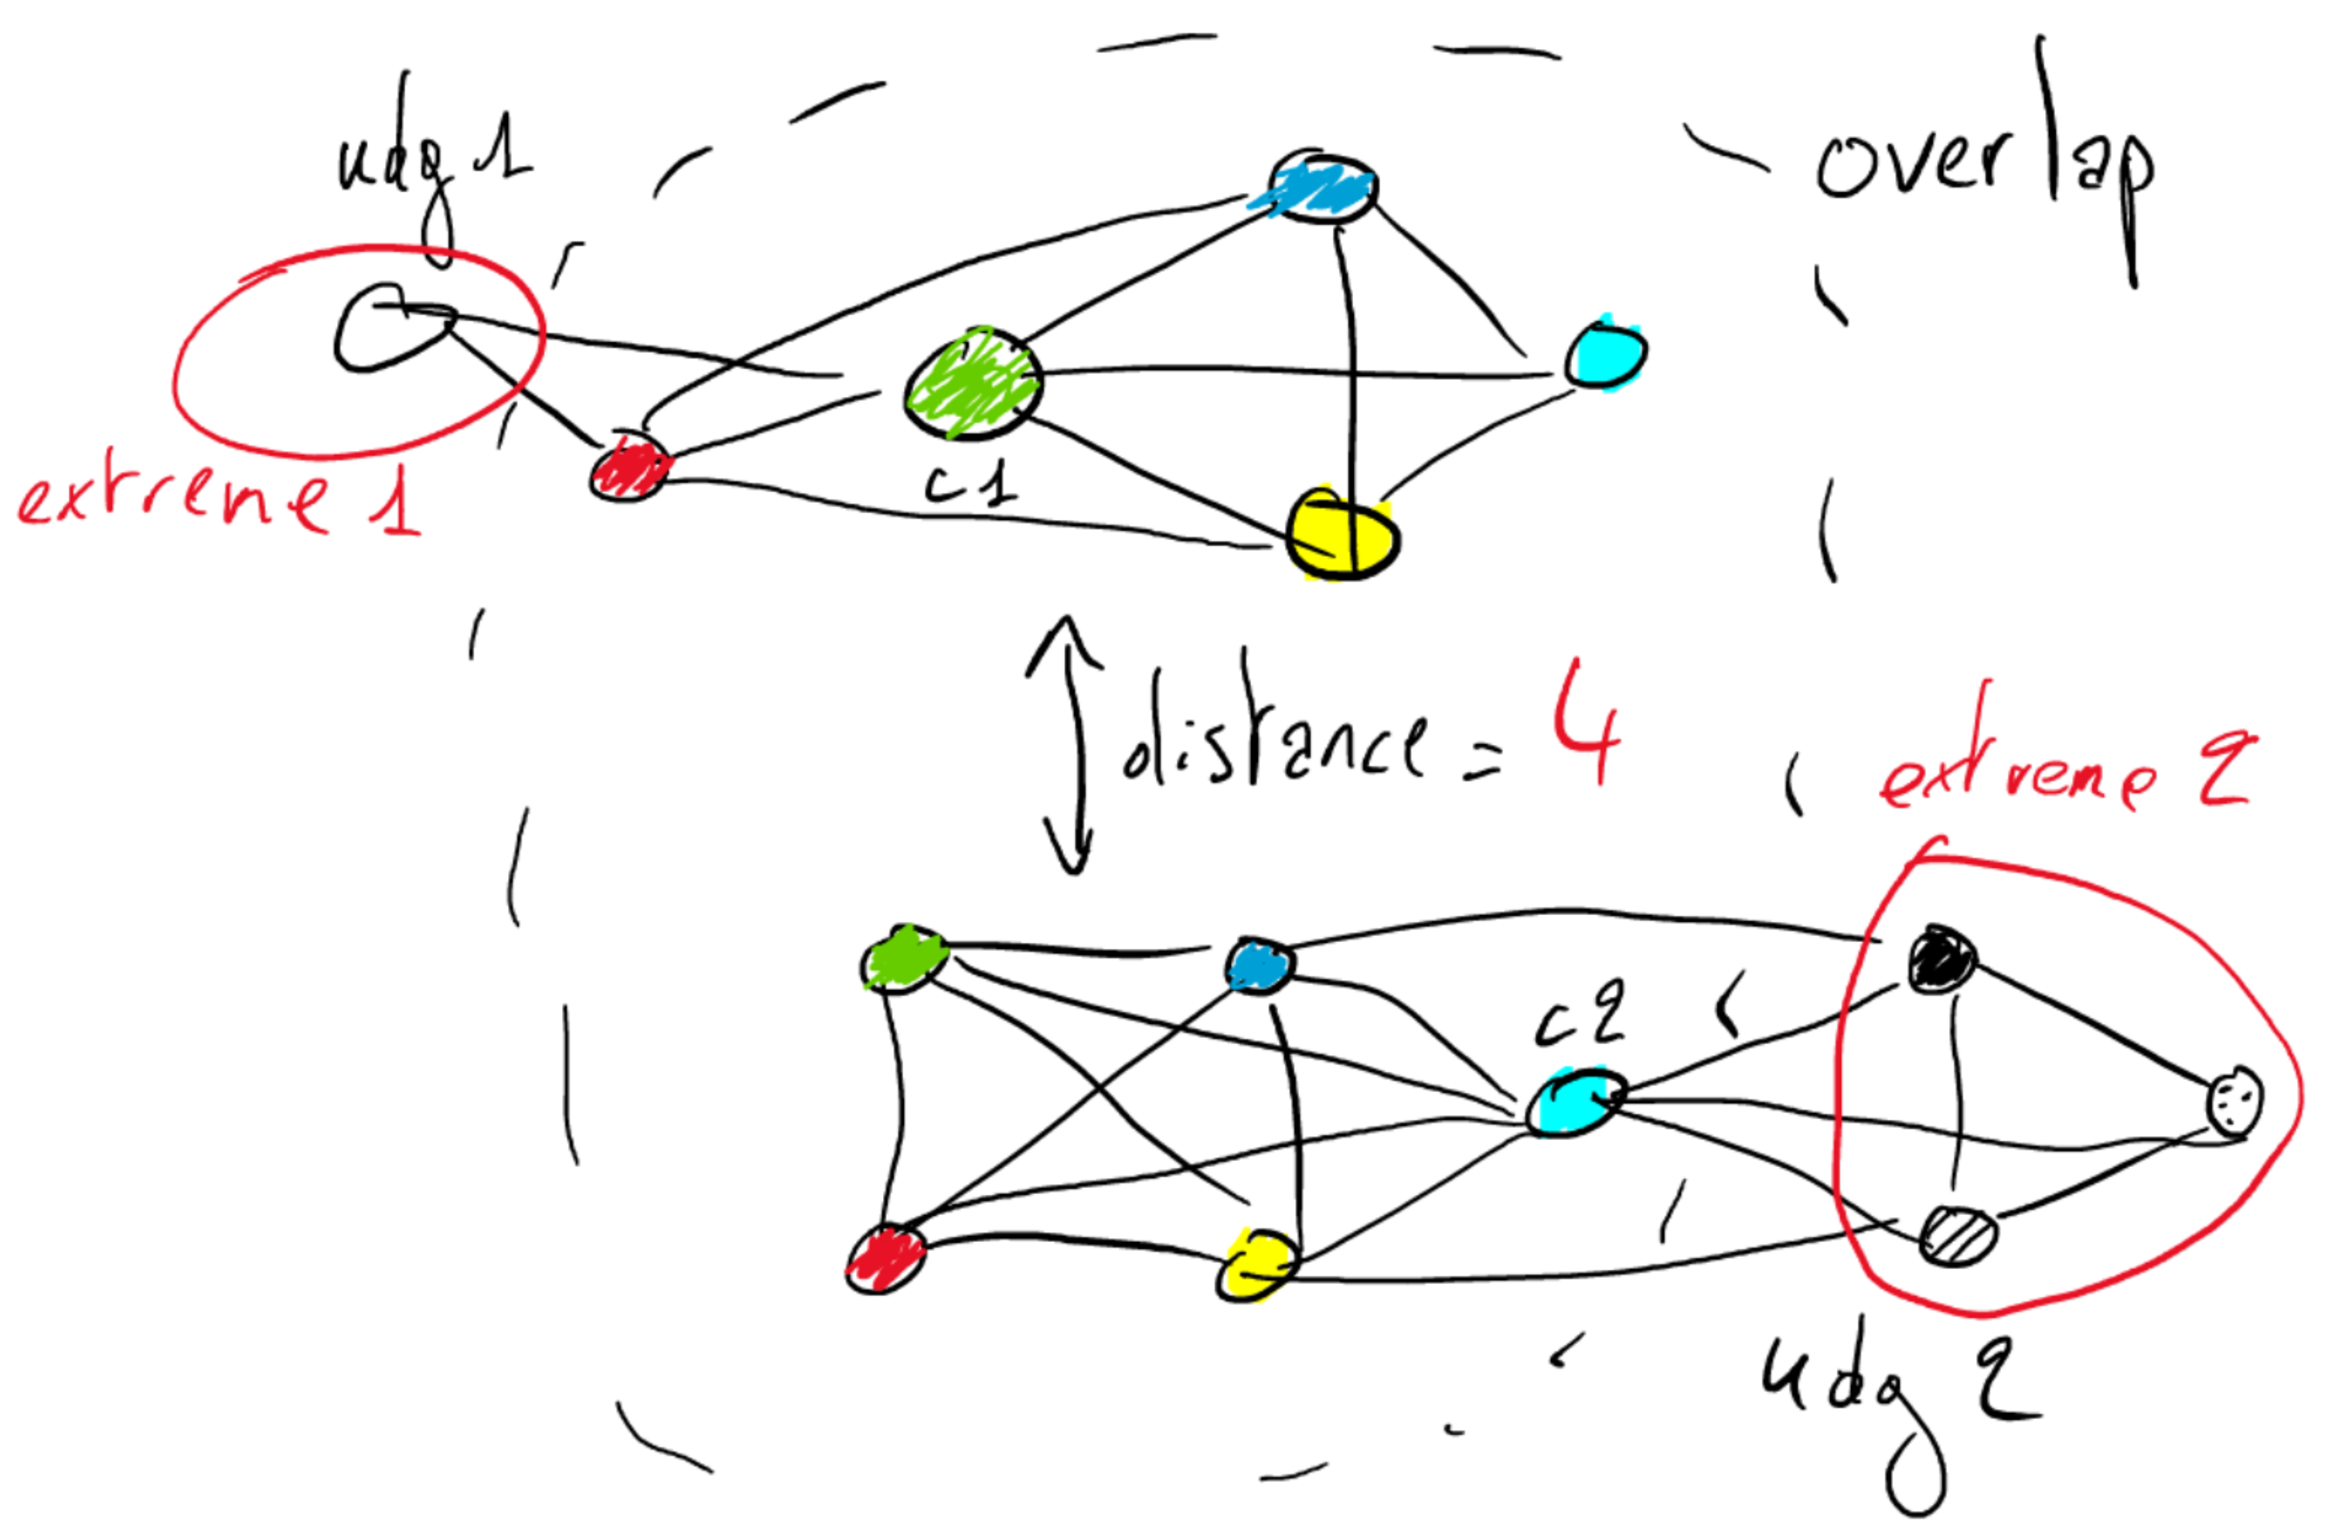
\includegraphics[width=0.6\textwidth]{overlap.pdf}
    \caption{Unit $d$-graph overlap}
    \label{fig:overlap}
\end{figure}

A real barcode graph is a bit more messy and two successive udgs can have different sizes, share less than $2 \times d$ barcodes and have more than 2 extreme nodes (Fig \ref{fig:overlap}.
But the idea remain the same, we should be able to go from the first udg (regarding the genomic position) to the last one by successive overlaps.

To support this traversal operation, we create a graph of unit $d$-graphs that we call $d^2$-graph (d2g).
In this graph, the nodes are the udgs generated by the algorithm \ref{algo:audg} and the edges are weighted edges between udgs that share at least one barcode.
The weight (distances) are defined as the number of barcodes that are extreme nodes separating the udgs pairs (Fig \ref{fig:overlap}.

TODO: Voir avec Rayan pour utilisation threshold/moyen plus malin.


Interesting assembly properties.
Cedric work on path retrieving ?
conclusion: More interesting solution for counting problem (filter out a lot of wrong udgs).
Assembly process allow to traverse the graph and try to extract total order.